\section{Rachunek \(\lambda\) z typami prostymi}
Przedstawimy system rachunku \(\lambda\) z typami prostymi w stylu de Bruijna \cite{barendregt_dekkers_statman_2013, Urzyczyn2006}. Zgodnie z \cite[roz. 13E]{Hindley:2008:LCI:1388400} odpowiada on najsłabszemu z \emph{czystych systemów typów}  (ang. \emph{pure type systems}, PTS) w myśl klasyfikacji zaproponowanej przez Henka Barendregta w \cite{barendregt_1991}. Klasyfikację tę obrazuje Rysunek \ref{fig:lambda-cube}; kierunek krawędzi oznacza na nim zawieranie w sensie możliwości wyrażenia słabszego systemu przez system wzbogacony o nowe typy.

\begin{figure}[h]
\centering
\begin{tikzpicture}
\matrix (m) [matrix of math nodes,
row sep=3em, column sep=3em,
text height=1.5ex,
text depth=0.25ex]{
            & \lambda\omega             &              & \lambda\Pi\omega             \\
\lambda 2   &                           & \lambda\Pi 2                                \\
            & \lambda\underline{\omega} &              & \lambda\Pi\underline{\omega} \\
\lambda{\to}&                           & \lambda\Pi  \\
};
\path[-{Latex[length=2.5mm, width=1.5mm]}]
(m-1-2) edge (m-1-4)
(m-2-1) edge (m-2-3)
        edge (m-1-2)
(m-3-2) edge (m-1-2)
        edge (m-3-4)
(m-4-1) edge (m-2-1)
        edge (m-3-2)
        edge (m-4-3)
(m-3-4) edge (m-1-4)
(m-2-3) edge (m-1-4)
(m-4-3) edge (m-3-4)
        edge (m-2-3);
\end{tikzpicture}
\caption{Kostka lambda H. Barendregta}
\end{figure}\label{fig:lambda-cube}

%System \(\lambda_{\to}\) w stylu Churcha to zbiór typów \(\mathrm{T}\),
%zbiór pseudotermów \(\Lambda_{\mathrm{T}}\), rodzina otoczeń typowych,
%relacja \(\beta\)-kontrakcji \(\to_{\beta}\) i relacja przypisania typu \(\vdash\).

\subsection{Typy proste}\label{ssec:typy-proste}
Niech \(\mathrm{U}\) będzie przeliczalnie nieskończonym zbiorem zmiennych przedmiotowych \(p,\ q,\ \dots\ \) (być może indeksowanych liczbami naturalnymi), które będziemy nazywali \emph{zmiennymi typowymi}.\begin{definicja}\label{def:typy-proste}(Typy proste)\\
\emph{Typami prostymi} będziemy określali najmniejszy w sensie mnogościowym zbiór wyrażeń taki, że:
\begin{enumerate}[label=T\arabic*.]
  \item Jeśli \(p\) jest zmienną typową, to \(p\) jest typem prostym.\label{def:t-1}
  \item Jeśli \(\tau\) i \(\sigma\) są typami prostymi, to \(\left(\tau\to\sigma\right)\) jest typem prostym.\label{def:t-2}
\end{enumerate}
\end{definicja}

Typy proste zbudowane tylko wedle reguły \ref{def:t-1} nazywamy typami \emph{atomowymi}, zaś wyrażenia zbudowe wedle reguły \ref{def:t-2} -- typami \emph{funkcyjnymi}. Zbiór typów prostych określony w myśl powyższej definicji będziemy oznaczali przez \(\mathbf{T_\to}\).

Późniejsze litery alfabetu greckiego, tj. \(\sigma,\, \tau,\, \rho,\ \dots\) będą służyły nam za zmienne metasyntaktyczne do oznaczania typów prostych. Dla lepszej czytelności będziemy pomijali najbardziej zewnętrzne nawiasy. Konstruktor typu \(\to\) wiąże prawostronnie; oznacza to, że typy \(\tau\to\sigma\to\theta\) oraz \(\tau\to(\sigma\to\theta)\) będziemy uznawali za tożsame.

Typy proste ujęte Definicją \ref{def:typy-proste} mają strukturę drzewa binarnego. Wysokość takiego drzewa będziemy nazywali \emph{stopniem} typu. Precyzyjnie ujmuje to pojęcie poniższa definicja.
\begin{definicja}\label{def:stopien-typu}(Stopień typu)\\
  Stopniem typu nazywamy funkcję \(\delta :\: \mathbf{T}_\to \longrightarrow \mathbb{N}\) taką, że
  \begin{align*}
    \delta(p) &= 0,\ \text{gdzie \(p\) jest typem atomowym},\\
    \delta(\tau\to\sigma)&=1 + \max\left(\delta(\tau),\ \delta(\sigma)\right).
  \end{align*}
\end{definicja}

\subsection{Pseudotermy}
  Niech \(\mathrm{V}\) będzie przeliczalnie nieskończonym zbiorem zmiennych przedmiotowych \(x,\ y,\ \dots\ \) (indeksowanych być może liczbami naturalnymi). Elementy takiego zbioru będziemy nazywali \emph{\(\lambda\)-zmiennymi}.
\begin{definicja}(Pseudo-pretermy)\\
  \emph{Pseudo-pretermami} będziemy nazywali najmniejszy (w sensie mnogościowym) zbiór \(\mathbf{\tilde\Lambda}_{\mathrm{T}}\) taki, że:

\begin{enumerate}[label=PT\arabic*.]
  \item Jeśli \(x\in \mathrm{V}\), to \(x\in{\mathbf{\tilde\Lambda}}_{\mathrm{T}}\).\label{def:pt-1}
  \item Jeśli \(M\in\mathbf{\tilde{\Lambda}}_{\mathrm{T}}\) i \(N\in\mathbf{\tilde{\Lambda}}_{\mathrm{T}}\), to \((MN)\in\mathbf{\tilde{\Lambda}}_{\mathrm{T}}\).\label{def:pt-2}
  \item Dla dowolnych \(x\in \mathrm{V}\), \(\sigma\in\mathbf{T}_\to\), \(M\in\mathbf{\tilde{\Lambda}}_{\mathrm{T}}\) mamy, że \((\lambda x^{\sigma}.\,M)\in \mathbf{\tilde{\Lambda}}_{\mathrm{T}}\).\label{def:pt-3}
  \end{enumerate}
\end{definicja}
  Wyrażenia postaci \ref{def:pt-2} nazywamy \emph{aplikacjami} \(M\) do \(N\), zaś wyrażenia postaci \ref{def:pt-3} -- \emph{\(\lambda\)-abstrakcjami}, gdzie o wszystkich podtermach termu \(M\) mówi się, że są w \emph{zasięgu} \(\lambda\)-abstraktora, zaś o \(\lambda\)-zmiennej \(x\) mówi się, że jest nim \emph{związana}.

  Za zmienne metasyntaktyczne obieramy duże litery alfabetu łacińskiego \(M,\ N,\ \dots\ \) Podobnie jak w podrozdziale \ref{ssec:typy-proste} stosujemy konwencję o opuszczaniu najbardziej zewnętrznych nawiasów. Aplikacja termów wiąże lewostronnie; oznacza to, że będziemy utożsamiali ze sobą wyrażenia \(MNP\) oraz \((MN)P\).

\newpage

\begin{definicja}(Zmienne wolne)
  \item Dla pseudo-pretermu \(M\) określamy zbiór \emph{pseudo-pretermów wolnych} \(\mathrm{FV}\) w nastepujący sposób:
    \begin{align*}
      \mathrm{FV}(x) &= \{x\}\\
      \mathrm{FV}(\lambda x^\sigma .\, P)  &= \mathrm{FV}(P)\setminus\{x\}\\
      \mathrm{FV}(P Q) &= \mathrm{FV}(P)\cup\mathrm{FV}(Q)
    \end{align*}
Jesli \(\mathrm{FV}(M)=\emptyset\), to mówimy, że \(M\) jest \emph{domknięcite}.
\end{definicja}
%  \item Podstawieniem pseudotermu \(N\) za \(\lambda\)-zmienną \(x\) w pseudotermie \(M\), symbolicznie \(M[x/N]\), nazywamy przekształcenie pseudotermu zadane następującymi warunkami:
%    \begin{enumerate}[label=({\alph*})]
%    \item Podstawienie jest poprawne wtedy i tylko wtedy, gdy żadne wolne wystąpienie \(\lambda\)-zmiennej \(x\) w pseudotermie \(M\) nie występuje w podtermie \(M\) postaci \(\lambda y.\, L\), gdzie \(y\in\mathrm{FV}(N)\).
%    \item
%      \begin{align*}
%        x[x/N] &= N,&\\
%        y[x/N] &= y,\ &\text{o ile}\ x\neq y,&\\
%        (PQ)[x/N] &= P[x/N]\,Q[x/N],&\\
%        (\lambda x.\,P)[x/N] &= \lambda x.\,P,&\\
%        (\lambda y.\,P)[x/N] &= \lambda y.\,P [x/N],\ &\text{o ile}\ x\neq y.
%      \end{align*}
%    \end{enumerate}

\begin{definicja}(Podstawienie)\\
\emph{Podstawieniem} \([x/N]\) pseudo-pretermu \(N\) za \(\lambda\)-zmienną \(x\) w \(M\) nazwamy zdefiniowane następująco przekształcenie:
  \begin{align*}
    x[x/N] &= N,\\
    y[x/N] &= y,\ &\text{o ile}\ x\neq y,\\
    (PQ)[x/N] &= P[x/N]\,Q[x/N],\\
    (\lambda y^\sigma.\, P)[x/N] &= \lambda y^\sigma .\,P[x/N],\ &\text{gdzie}\ x\neq y\ \text{i}\ y\not\in \mathrm{FV}(N).\\
  \end{align*}
\end{definicja}

\noindent Zachodzą następujące fakty:
    \begin{fakt}
      \begin{enumerate}[label=({\alph*})]
        \item Jeśli \(x\not\in\mathrm{FV}(M)\), to \(M[x/N]\) jest poprawnym podstawieniem i \(M[x/N]=M\).
        \item Jeśli \(M[x/N]\) jest poprawnym podstawieniem, to \(y\in\mathrm{FV}(M[x/N]\) wtw, gdy albo \(y\in\mathrm{FV}(M)\)
          i \(x\neq y\), albo \(y\in \mathrm{FV}(N)\) i \(x\in \mathrm{FV}(M)\).
        \item Podstawienie \(M[x/x]\) jest poprawne i \(M[x/x]=M\).
        \item Jeśli \(M[x/y]\) jest poprawnym podstawieniem, to \(M[x/y]\) ma tę samą długość, co \(M\).
      \end{enumerate}
    \end{fakt}
    \begin{fakt}
      Powiedzmy, że \(M[x/N]\) jest poprawnym podstawieniem i \(N[y/L]\) i \(M[x/N][y/L]\) są poprawnymi podstawieniami, gdzie
      \(x\neq y\). Jeśli \(x\not\in \mathrm{FV}(L)\) lub \(y\not\in\mathrm{FV}(M)\), to \(M[y/L]\) i \( M[y/L]\left[x/N[y/L]\right] \) jest poprawnym podstawieniem oraz
      \[
        M[x/N][y/L]=M[y/L][x/N[y/L]].
      \]
    \end{fakt}

    \begin{fakt}
      Jesli \(M[x/y]\) jest poprawnym postawieniem i \(y\not\in\mathrm{FV}(M)\), to \(M[x/y][y/x]\) jest poprawnym podstawieniem oraz
      \(M[x/y][y/x]=M\).
    \end{fakt}

  \begin{definicja}(\(\alpha\)-konwersja)\\
    \(\alpha\)-konwersją nazywamy najmniejszą (w sensie mnogościowym) zwrotną i przechodnią relację binarną \(=_\alpha\) określoną na zbiorze pseudotermów \(\mathbf{\tilde{\Lambda}}_{\mathrm{T}}\) spełniającą poniższe warunki:
    \begin{enumerate}[label=({\alph*})]
      \item Jeśli \(y\not\in \mathrm{FV}(M)\) i \(M[x/y]\) jest poprawnym podstawieniem, to \(\lambda x.\, M  =_\alpha \lambda y.\, M[x/y]\).
      \item Jeśli \(M=_\alpha N\), to dla każdej \(\lambda\)-zmiennej \(x\) mamy \(\lambda x.\, M =_\alpha \lambda x.\,N\).
      \item Jeśli \(M=_\alpha N\), to \(M Z=_\alpha N Z\).
      \item Jeśli \(M=_\alpha N\), to \(ZM =_\alpha ZN\).
    \end{enumerate}
  \end{definicja}

    \begin{fakt}
      Relacja \(=_{\alpha}\) jest symetryczna.
    \end{fakt}
    \begin{fakt}
      \(=_{\alpha}\) jest relacją równoważności.
    \end{fakt}
    \begin{fakt}
      Jeśli \(M=_\alpha N\), to \(\mathrm{FV}(M)=\mathrm{FV}(N)\).
    \end{fakt}

Dysponując powyższymi rozstrzygnięciami otrzymujemy wygodne utożsamienie pseudo-pretermów,
które różnią się między sobą tylko zmiennymi związanymi.

\begin{definicja}(Pseudotermy)\\
  Klasy abstrakcji relacji \(\alpha\)-konwersji nazywamy \emph{pseudotermami}. Zbiór wszystkich pseudotermów oznaczamy następująco:
\[
  \mathbf{\Lambda}_{\mathrm{T}}=\left\{[M]_\alpha\:|\: M\in\mathbf{\tilde{\Lambda}}_\mathrm{T}\right\}
\]
\end{definicja}
Nadużywając notacji będziemy odnosili się do pseudotermów tylko przez ich reprezentantów: zamiast \([\lambda x^\sigma. M]_{\alpha}\) będziemy pisali krótko \(\lambda x^\sigma. M\).
\subsection{Typowalność}
%\item
%  \emph{Pseudo-pretermami} nazywamy język \(\Lambda_{\mathrm{T}}\) generowany przez
%gramatykę 
%\[
%  \Lambda^{-}_{\mathrm{T}} := \ \mathrm{V}\ | \ \left (\lambda V^{\mathrm{T}} . \Lambda^{-}_{\mathrm{T}}\right) \ | \ \left (\Lambda^{-}_{\mathrm{T}}\Lambda^{-}_{\mathrm{T}}\right)
%\]
%    gdzie V to przeliczalny zbiór \(\lambda\)-zmiennych \(x, y, \dots\)

%    W języku podmiotowym będziemy używali późniejszych liter alfabetu łacińskiego pisanych kursywą (\(M,\, N,\, O,\, \dots\)) oznaczając pseudotermy.

\begin{definicja}(Kontekst)\\
  \emph{Kontekstem} nazywamy skończoną funkcję częściową \(\Gamma:\:\mathrm{V}\longrightarrow\mathbf{T_\to}\), czyli zbiór par postaci \(\Gamma=\{x_1^{\tau_1},\,\dots,\,x_n^{\tau_n}\},\ \text{gdzie}\ (x_i^{\tau_i})=(x_i,\, \tau_i)\ \text{oraz}\ x_i \neq x_j\ \text{dla}\ i\neq j\). Zbiór
  \[\mathrm{dom}(\Gamma) = \left\{x\in \mathrm{V}\,|\,\exists\tau(x^\tau\in\Gamma)\right\}\]
  nazywamy \emph{dziedziną} kontekstu \(\Gamma\), zaś
  \[\mathrm{rg}(\Gamma)=\left\{\tau\in\mathbf{T}_\to\,|\,\exists x(x^\tau\in\Gamma)\right\}\]
  -- \emph{zakresem} kontekstu \(\Gamma\).
  Piszemy:
  \begin{easylist}
    & \(x_{1}^{\tau_1},\,x_{2}^{\tau_2}\) zamiast \(\{x_{1}^{\tau_1},\, x_{2}^{\tau_2}\}\), o ile \(x_{1}^{\tau_1}\) i \(x_{2}^{\tau_2}\) są różne,
    & \(\Gamma,\, x^\tau\) zamiast \(\Gamma\cup \{x^\tau\}\), o ile \(x^\tau\not\in \Gamma\),
    & \(\Gamma,\, \Delta\) zamiast \(\Gamma\cup \Delta\), o ile \(\Gamma\cap\Delta=\emptyset\).
  \end{easylist}
\end{definicja}

Okreslimy teraz system przypisywania typów do pseudotermów w stylu dedukcji naturalnej. \emph{Sekwentami} w tym systemie będziemy nazywali wyrażenia postaci \(\Gamma\vdash M^{\sigma}\), gdzie \(M\in\mathbf{\Lambda}_{\mathrm{T}},\ \sigma\in\mathbf{T_\to}\), zaś \(\Gamma\) jest pewnym kontekstem.

Wprowadzamy następujące reguły dowodzenia:
    \begin{center}
    \begin{tabular}{ ccc}
      {\begin{prooftree}
        \Hypo{}
        \Infer1[(Var)]{\Gamma, x^\tau\vdash x^\tau}
      \end{prooftree}},
      &
      {\begin{prooftree}
        \Hypo{ \Gamma, x^{\varphi} \vdash M^{\psi} }
        \Infer1[(Abs)]{\Gamma \vdash (\lambda\, x^{\varphi}.\, M)^{\varphi\to\psi}}
      \end{prooftree}},
      &
      {\begin{prooftree}
        \Hypo{\Gamma \vdash M^{\varphi \to \psi}} \Hypo{ \Gamma \vdash N^{\varphi}}
        \Infer2[(App)]{\Gamma \vdash (MN)^{\psi}}
      \end{prooftree}}.
      \end{tabular}
    \end{center}

\begin{definicja}(Typowalność)\\
  Mówimy, że pseudoterm \(M\) jest typu \(\sigma\) w kontekście \(\Gamma\) (jest \emph{typowalny}), jeśli istnieje skończone drzewo sekwentów spełniające poniższe warunki:
  \begin{enumerate}[label=P\arabic*.]
      \item W korzeniu drzewa znajduje się sekwent \(\Gamma \vdash M^\sigma\).
      \item Liście są \emph{aksjomatami}, tj. sekwentami postaci \(\Gamma, x^\sigma \vdash x^\sigma\).
      \item Każdego rodzica można otrzymać z jego dzieci przez zastosowanie którejś z reguł wyprowadzania nowych sekwentów.
  \end{enumerate}
  Tak określone drzewo będziemy nazywali \emph{wyprowadzeniem} typu i pisali \(\Gamma \vdash M^\sigma\).

Otrzymujemy ostateczne określenie \(\lambda\)-termów w omawianym systemie.

\begin{definicja}\label{def:lambda-term}(\(\lambda\)-termy)\\
   Wszystkie typowalne pseudotermy w pewnym kontekście \(\Gamma\) nazywamy \emph{\(\lambda\)-termami} (z typami prostymi w  kontekście \(\Gamma\)).
  \begin{uwaga*}
\(\lambda\)-term w kontekście \(\Gamma_1\) może nie być typowalny w innym kontekście \(\Gamma_2\).
  \end{uwaga*}
\end{definicja}

  Zachodzą następujące fakty:
  \begin{fakt}(o odwracaniu)
  \begin{enumerate}[label=I\arabic*.]
    \item Jeśli \(\Gamma \vdash x^\sigma\), to \(x^\sigma\in\Gamma\).\label{thm:i-1}
    \item Jeśli \(\Gamma \vdash MN^\sigma\), to istnieje typ \(\tau\in\mathbf{T_\to}\) taki, że
          \(\Gamma\vdash M^{\tau\to\sigma}\) i \(\Gamma\vdash N^\tau\).\label{thm:i-2}
    \item Jesli \(\Gamma \vdash \lambda x^\tau .\, M^\sigma\), to istnieje typ \(\rho\in\mathbf{T}_\to\) taki, że
          \(\sigma\equiv \tau\to\rho\) oraz \(\Gamma,\, x^\tau \vdash M^\rho\).\label{thm:i-3}
  \end{enumerate}
  \begin{dowod}
  \ref{thm:i-1} Przypuśćmy, że \(\Gamma\vdash x^\sigma\). Ostatni wierzchołek w wyprowadzeniu nie może być uzyskany przez żadne z określonych reguł dowodzenia, zatem musi to być aksjomat, tj. \(x^\sigma\in\Gamma\). Podobnie \ref{thm:i-2} i \ref{thm:i-3}.\qed
  \end{dowod}
  \end{fakt}

  \begin{fakt}(o podstawianiu)
      Jeśli \(\Gamma,\,x^\sigma\vdash M^\tau\) oraz \(\Gamma \vdash N^\sigma\), to
            \(\Gamma \vdash M[x/N]^\tau\).
      \begin{dowod}
      Dowód przez indukcję strukturalną względem M. \qed
      \end{dowod}
  \end{fakt}
  W danym kontekście każdy \(\lambda\)-term ma jednoznacznie przypisany typ, co stwierdza następujące twierdzenie:
\end{definicja}

\begin{fakt}\label{thm:jedoznacznosc-typu}
Jesli \(\Gamma\vdash M^\sigma\) oraz \(\Gamma\vdash M^\tau\), to \(\sigma=\tau\).
\begin{dowod}
  Dowód przez indukcję strukturalną względem M. \qed
\end{dowod}
\end{fakt}

\begin{uwaga}(Adnotacje typowe)
  Mówiąc o \(\lambda\)-termach i nie podając żadnego związanego z nimi kontekstu \(\Gamma\) będziemy implicite zakładali, że istnieje pewien kontekst w którym są one typowalne. Wspólny dla \(\lambda\)-termów \(M^\sigma\) i \(N^\tau\) kontekst \(\Gamma\) będziemy notowali pisząc \(M,\ N\in\mathbf{\Lambda}^{\Gamma}_{\mathbf{T}}\). Ze względu na Fakt \ref{thm:jedoznacznosc-typu} mając określony kontekst \(\Gamma\) będziemy bez utraty jednoznaczności omijać adnotacje typowe dla \(\lambda\)-termów pisząc po prostu \(M\) w miejsce \(M^\sigma\), gdy z kontekstu jasne będzie, że nie chodzi o pseudotermy.

  Typ dowolnego \(\lambda\)-termu będziemy w ramach konwencji notowali używając adnotacji typowej umieszczonej w górnym indeksie. Dla przykładu, pisząc \(\left(M^{\sigma\to\tau}N^\sigma\right)^\tau\) będziemy mieli na myśli, że \(\lambda\)-term jest w pewnym kontekście \(\Gamma\) typu \(\tau\). \end{uwaga}

Rozważmy następujące przykłady:
\begin{przyklad}
  Niech \(\Gamma=\{x^\sigma,\, y^\tau\}\). Pokażemy, że \(\mathrm{K}=\lambda x^\sigma y^\tau .\, x\) ma typ \(\sigma\to\tau\to\sigma\). Istotnie,
  \begin{center}
  \begin{prooftree}
    \Hypo{x^\sigma, y^\tau \vdash x^\sigma}
    \Infer1[(Abs)]{x^\sigma \vdash (\lambda y^\tau.\,x)^{\tau\to\sigma}}
    \Infer1[(Abs)]{\vdash (\lambda x^\sigma \lambda y^\tau .\, x)^{\sigma\to\tau\to\sigma}}
\end{prooftree}
  \end{center}
\end{przyklad}

\begin{przyklad}
  Niech \(\Gamma=\{x^{\tau\to\rho},\, y^{\sigma\to\tau},\,z^{\sigma}\}\). Wówczas
  \begin{center}
\begin{prooftree}
  \Hypo{ \Gamma \vdash z^{\sigma}} \Hypo{\Gamma \vdash y^{\sigma\to\tau}}
  \Infer2[(App)]{\Gamma \vdash yz^{\tau}}
  \Hypo{\Gamma\vdash x^{\tau\to\rho}} \Infer2[(App)]{\Gamma \vdash x(yz)^\rho}
  \Infer1[(Abs)]{x^{\tau\to\sigma}, y^{\sigma\to\rho}\vdash (\lambda z^\sigma .\, x(yz))^{\sigma\to\rho}}
  \Infer1[(Abs)]{x^{\tau\to\rho}\vdash (\lambda y^{\sigma\to\tau} \lambda z^{\sigma}.\,x(yz))^{(\sigma\to\tau)\to\sigma\to\rho}}
  \Infer1[(Abs)]{\vdash (\lambda x^{\tau\to\rho} \lambda y^{\sigma\to\tau} \lambda z^\sigma .\, x(yz))^{(\tau\to\rho)\to(\sigma\to\tau)\to\sigma\to\rho}}
\end{prooftree}
  \end{center}
  Zauważmy, że term \(\lambda x^{\tau\to\rho}\lambda y^{\sigma\to\tau}\lambda z^\sigma . x(yz)\) odpowiada operacji złożenia funkcji.
  %Co więcej, można wykazać że typ \((\tau\to\rho)\to(\sigma\to\tau)\to\sigma\to\rho\) może mieć tylko i wyłącznie operacja złożenia~\cite{Wadler1989}.
\end{przyklad}
\begin{uwaga}\label{rm:skonczonosc-lambdatermow}
Widzimy, że wyprowadzanie typu odpowiada w gruncie rzeczy konstrukcji \(\lambda\)-termu. Ponieważ każde wyprowadzenie musi być skończone, typowalne są tylko pseudotermy skończonej długości.
\end{uwaga}
\begin{przyklad}\label{ex:omega-kombinator}
  Nie wszystkie pseudotermy są typowalne w rachunku \(\lambda\) z typami prostymi.
  Istotnie, przypuśćmy że \(\omega=(\lambda x^{\sigma\to\sigma} .\, x x)\) jest typowalny. Wówczas dla kontekstu \(\Gamma\) mamy \(x^{\sigma\to\sigma}\in\Gamma\). Ponieważ \(\omega\) zawiera w sobie podterm \((xx)\), to w wyprowadzeniu musiał on zostać otrzymany przez zastosowanie reguły (App). Wówczas \(x^\sigma \in \Gamma\)  i \(x^{\sigma\to\sigma} \in \Gamma\), co nie jest możliwe, bo \(\Gamma\) musiałby nie być prawidłowo określonym kontekstem.
\end{przyklad}

Przykład \ref{ex:omega-kombinator} wskazuje, że rachunek \(\lambda\) z typami prostymi nie ma wystarczających środków wyrazu, aby definiować w nim funkcje rekurencyjne. W rachunku \(\lambda\) bez typów definicje takie są osiągane za pomocą \emph{kombinatorów punktu stałego}, które w rachunku \(\lambda\) z typami prostymi nie są typowalne właśnie ze względu na fakt, że nie jest możliwe wyprowadzenie typu dla aplikacji termu do samego siebie.

\subsection{Redukcja}
\begin{definicja}(Zgodność)\\
  Relację \(\mathrm{R}\) na zbiorze pseudotermów \(\mathbf{\tilde\Lambda}_{\mathrm{T}}\) nazywamy \emph{zgodną}, jeśli dla \(M,\,N,\,Z\in\mathbf{\tilde\Lambda}_{\mathrm{T}}\) spełnia ona następujące warunki:
  \begin{enumerate}[label=\roman*)]
    \item Jeśli \(M\mathrm{R} N\), to \((\lambda x^\sigma.\,M)\, \mathrm{R}\, (\lambda x^\sigma.\, N)\) dla dowolnych \(x\in \mathrm{V}\) i \(\sigma\in \mathbf{T_\to}\).
    \item Jeśli \(M\mathrm{R} N\), to \((MZ)\,\mathrm{R}\, (NZ)\).
    \item Jeśli \(M\mathrm{R} N\), to \((ZM)\,\mathrm{R}\, (ZN)\).
  \end{enumerate}
Przy powyższych ustaleniach \emph{kongruencją} będziemy nazywali każdą zgodną relację równowazności na \(\mathbf{\tilde\Lambda}_{\mathrm{T}}\), zaś \emph{redukcją} – każdą zgodną, zwrotną i przechodnią relację na \(\mathbf{\tilde\Lambda}_{\mathrm{T}}\).
\end{definicja}

\begin{definicja}(\(\beta\)-redukcja)\\
  \(\beta\)-redukcją nazywamy najmniejsza w sensie mnogościowym \emph{zgodną} relację binarną \(\longrightarrow_{\beta}\) określoną zbiorze na pseudotermów \(\mathbf{\tilde\Lambda}_{\mathrm{T}}\) za pomocą podstawienia
  \[
    (\lambda x^\sigma.\,P)Q \longrightarrow_{\beta} P[x/Q].
  \]

  \emph{\(\beta\)-redeksami} bedziemy nazywali wyrażenia postaci \((\lambda x^\sigma.\, M)N\), zaś rezultat ich \(\beta\)-redukcji w postaci termu \(M[x/N]\) -- \emph{\(\beta\)-reduktem}.

  Nadużywając notacji, z każdym \(\beta\)-redeksem \(\Delta\) postaci \((\lambda x^\tau .\,P^\rho)R\) będziemy wiązali jego \emph{stopień} i pisali \(\delta((\lambda x^\tau .\,P^\rho)R)=\delta(\tau\to\rho)\), gdzie występująca po prawej stronie równości \(\delta\) jest określona w myśl Definicji \ref{def:stopien-typu}. Dysponując tą konwencją możemy określić pojęcie stopnia dowolnego \(\lambda\)-termu.

\begin{definicja}\label{def:stopien-termu}(stopień \(\lambda\)-termu)\\
  Stopniem \(\mathrm{d}(M)\) \(\lambda\)-termu \(M\) nazywamy supremum zbioru stopni \(\beta\)-redeksów, które są zawarte w \(M\), czyli
  \[\mathrm{d}(M)=\sup\{\delta(N) \:|\:N\ \text{jest \(\beta\)-redeksem w}\ M\}.\]
\end{definicja}

\begin{uwaga*}
  Z każdym \(\beta\)-redeksem \(\Delta\) związane są więc dwa rodzaje stopni: stopień \(\mathrm{d}(\Delta)\) jako \(\lambda\)-termu w myśl Defnicji \ref{def:stopien-termu} i stopień \(\beta\)-redeksu \(\delta(\Delta)\).
\end{uwaga*}

%\begin{lemat}
%  Niech \(M\) i \(N\) będą dowolnymi \(\lambda\)-termami w kontekście \(\Gamma\) takimi, że \(x\in\mathrm{FV}(M)\) i \(x^\tau \in \Gamma\). Wówczas \(\mathrm{d}(M[x/N])\leq \max\left\{\mathrm{d}(M),\, \mathrm{d}(N),\, \delta(\tau)\right\}\).
%\end{lemat}
%\begin{dowod}
%
%\end{dowod}

\end{definicja}
\noindent Określamy następujące relacje:
\begin{enumerate}[label=B\arabic*.]
  \item \(\longrightarrow^{+}_{\beta}\) jest przechodnim domknięciem relacji \(\longrightarrow_{\beta}\) w zbiorze pseudotermów \(\mathbf{\tilde\Lambda}_{\mathrm{T}}\).

  \item \(\longrightarrow^{*}_{\beta}\) jest domknięciem przechodnio-zwrotnim w \(\mathbf{\tilde\Lambda}_{\mathrm{T}}\) relacji \(\longrightarrow_{\beta}\) (jest \emph{redukcją}).

  \item \(=_{\beta}\) jest najmniejszą relację równowazności zawierającą relację \(\longrightarrow_{\beta}\) (jest \emph{kongruencją}).
\end{enumerate}

\begin{definicja}\label{def:postac-normalna}(Postać normalna)\\
  Powiemy, że \(\lambda\)-term \(M\) jest w \emph{postaci normalnej}, jeśli żadna z jego podformuł nie jest \(\beta\)-redeksem. Przez \(\mathrm{NF}_{\beta}\) będziemy oznaczali zbiór wszystkich \(\lambda\)-termów w postaci normalnej.
\end{definicja}
Definicję postaci normalnej można ująć w alternatywny sposób w postaci Faktu \ref{thm:postac-normalna-alt}.

\begin{fakt}\label{thm:postac-normalna-alt}
\(M\) \emph{ma postać normalną}, jeśli \(M=_{\beta}N\) dla pewnego \(N\), który jest w postaci normalnej.
\end{fakt}
\begin{uwaga*}
Fakt, że \(=_{\beta}\) jest relacją równoważności może rodzić pokusę, aby utożsamić  ze sobą wszystkie postacie normalne danego \(\lambda\)-termu. Z Twierdzenia \ref{thm:church-rosser} wynika jednak, że jest to zupełnie zbędne, bowiem o ile tylko \(\lambda\)-term jest normalizowalny, to wiemy, że posiada dokładnie jedną postać normalną i każde takie utożsamienie byłoby trywialne.
\end{uwaga*}

  \begin{definicja}(\(\eta\)-redukcja)\\
\(\eta\)-redukcją nazywamy najmniejszą (w sensie mnogościowym) \emph{zgodną} relację w \(\mathbf{\Lambda}_{\mathrm{T}}\) taką, że
  \[
    \lambda x^\sigma.\, Mx\longrightarrow_{\eta} M,
  \]
    o ile \(x\not\in \mathrm{FV}(M)\).
  \end{definicja}

Zdefiniowane powyżej  \(\beta\)- i \(\eta\)-redukcje zachowują typ, jak stwierdza Fakt \ref{thm:poprawnosc-redukcji}. Własność ta pozwala sensownie mówić o redukcji \(\lambda\)-termów.
%pomimo, że te relacje są zdefiniowane dla pseudotermów.
\begin{fakt}\label{thm:poprawnosc-redukcji}(o poprawności redukcji)
  Jeśli \(\Gamma\vdash M^\sigma\) i \(M\longrightarrow^{*}_{\beta\eta}N\), to
  \(\Gamma\vdash N^\sigma\).
  \begin{dowod}
  \cite[tw. 1B.14]{barendregt_dekkers_statman_2013}.
  \end{dowod}
\end{fakt}
\subsection{Normalizacja}
\noindent Powiemy, że \(\lambda\)-term \(M\) ma własność:
\begin{easylist}
  & \emph{(słabej) normalizacji} (symbolicznie: \(M\in\mathrm{WN_{\beta}}\)) wtedy i tylko wtedy, gdy istnieje ciąg \(\beta\)-redukcji rozpoczynający się od \(M\) i kończący się termem w postaci normalnej \(N\).
  &  \emph{silnej normalizacji} (symbolicznie: \(M\in\mathrm{SN_{\beta}}\)), jeśli wszystkie ciągi \(\beta\)-redukcji rozpoczynające się od \(M\) są skończone.
\end{easylist}
\begin{uwaga*}
Z powyższego określenia  widzimy, że własność \(\mathrm{SN}_{\beta}\) pociąga za sobą własność \(\mathrm{WN}_{\beta}\).
\end{uwaga*}
\begin{definicja}(Strategia redukcji)\\
  \emph{Strategią redukcji} nazywamy odwzorowanie \(F:\:\mathbf{\Lambda}_{\mathrm{T}}\longrightarrow\mathbf{\Lambda}_{\mathrm{T}}\) takie, że \(F(M)=M\), gdy \(M\) jest w postaci normalnej i \(M\longrightarrow_{\beta}F(M)\) w przeciwnym wypadku. Mówimy, że strategia \(F\) jest \emph{normalizująca}, jeśli dla każdego \(M\in \mathrm{WN_\beta}\) istnieje \(i\in\mathbb{N}\) takie, że \(F^i (M)\) jest w postaci normalnej.
\end{definicja}

Z puktu widzenia praktyki obliczeniowej istotny jest podział strategi redukcji ze względu na kolejność w jakiej redukowane będą podwyrażenia \(\lambda\)-termów. Wyróżniamy:
\begin{easylist}
  & strategie ścisłe (ang. \emph{strict}), w których każdy \(\lambda\)-term przed aplikacją jest redukowany do postaci normalnej,
  & strategie nieścisłe (ang. \emph{non-strict}), w których dopuszcza się aplikowanie \(\lambda\)-termów, które można dalej zredukować.
\end{easylist}

\begin{przyklad}
  Niech \(\mathrm{K}=\lambda xy.\,x\), \(\mathrm{I}=\lambda x.\,x\), \(0 = \lambda x y.\, y\). 
  Rozważmy następujące ciągi redukcji:

  \begin{enumerate}[label=({\alph*})]
    \item Redukcja strategią scisłą:\begin{multline*}
              \mathrm{KI}((\lambda mnxy.\, m x (n x y))0 0) \longrightarrow_\beta \mathrm{KI}((\lambda nxy.\, 0 x (n x y)) 0) \longrightarrow_\beta \\
              \longrightarrow_\beta \mathrm{KI}((\lambda xy.\, 0 x (0 x y)))\longrightarrow_\beta \mathrm{KI}((\lambda xy.\, 0 x y))\longrightarrow_\beta \mathrm{KI0})\longrightarrow_\beta \mathrm{I}
          \end{multline*}

    \item Redukcja strategią nieścisłą:
      \[\mathrm{KI}((\lambda mnxy.\, m x (n x y))0 0) \longrightarrow_\beta \mathrm{I}\]

  \end{enumerate}
\end{przyklad}
\begin{twierdzenie}\label{thm:wn}(\emph{Własność \(\mathrm{WN}_{\beta}\)}) Wszystkie \(\lambda\)-termy mają postać normalną.
\end{twierdzenie}
\begin{dowod}
  Pokażemy, że dla dowolnego \(\lambda\)-termu \(M\) istnieje normalizująca strategia redukcji.

  Oznaczmy przez \(\mathrm{R}_\beta(M)\) zbiór \(\beta\)-redeksów znajdujących się w \(M\). Jeśli \(M\in \mathrm{NF}_\beta\), to \(\mathrm{R}_\beta(M)=\emptyset\) i twierdzenie zachodzi w sposób trywialny. Jeśli \(M\not\in \mathrm{NF}_\beta\), to istnieje w \(M\) przynajmniej jeden \(\beta\)-redeks. Z Uwagi \ref{rm:skonczonosc-lambdatermow} \(M\) jest skończonej długości, więc \(\mathrm{R}_\beta(M)\) jest skończony. Możemy więc wybrać z \(M\) \(\beta\)-redeks znajdujący się (rozpoczynający się) w \(M\) najbardziej na prawo. Oznaczmy taki \(\beta\)-redeks przez \(\Delta\).

  Niech \(\delta_M\) będzie stopniem \(M\) (Definicja \ref{def:stopien-termu}). Ponieważ wiele redeksów w \(M\) może mieć ten sam stopień \(\delta_M\), przez \(n_M\) oznaczmy liczbę wystąpień redeksów stopnia \(\delta_M\) w \(M\).

  Niech \(F\) będzie strategią redukcji polegającą na \(\beta\)-redukowaniu redeksu \(\Delta\) wybranego jak wyżej i niech \(M'=F(M)\).
  Zauważmy, że \(n_M < n_{M'}\), gdyż strategia \(F\) eliminuje \(\Delta\) z \(M'\) i może prowadzić do powstania redeksów tylko mniejszego stopnia.
  Istotnie, ilość redeksów w \(M\) może zwiększyć się na skutek \(\beta\)-redukcji tylko w jeden z poniższych sposobów:
  \begin{enumerate}[label=\roman*)]
    \item powstanie nie występujących wcześniej redeksów.\label{itm:wn-1}
    \item powielenie już istniejących redeksów.
  \end{enumerate}

W przypadku \ref{itm:wn-1}
  \begin{figure}[htb]
  \centering
  \begin{subfigure}{0.55\textwidth}
    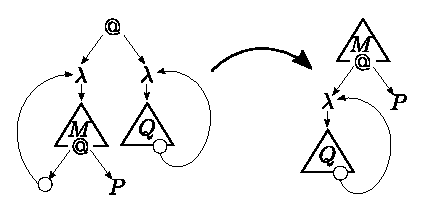
\includegraphics[width=1\linewidth]{../reduction1}
    \caption{Redukcja \((\lambda x^{\rho\to\mu}\overbrace{\dots\ .\,x P^\rho \dots}^{M^\tau})(\lambda y^\rho.\, Q^\mu)^{\rho\to\mu}\) do nowego redeksu \((\underbrace{\dots\ .\,(\lambda y^\rho.\,Q^\mu)P^\rho\dots}_{M[x/Q]^\tau})\).}
  \end{subfigure}


\end{figure}
\begin{figure}[htb]\ContinuedFloat
  \centering
  \vspace{1em}
  \begin{subfigure}{0.55\textwidth}
    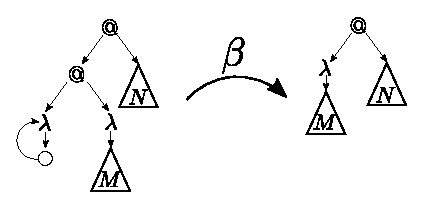
\includegraphics[width=1\linewidth]{../reduction2}
    \caption{Redukcja \((\lambda x^\tau \lambda y^\rho.\,P^\sigma)M^\tau N^\rho\) do nowego redeksu postaci \((\lambda y^\rho .\, P[x/M]^\sigma)N^\rho\).}
  \end{subfigure}


\end{figure}
\begin{figure}[htb]\ContinuedFloat
  \centering
  \begin{subfigure}{0.55\textwidth}
    \includegraphics[width=1\linewidth]{../reduction3}
    \caption{Redukcja \((\lambda x^{\tau\to\rho}.\,x)(\lambda y^\tau.\,M^\rho) N^\tau\) do nowego redeksu \((\lambda y^\tau.\,M^\rho)N^\tau\).}
  \end{subfigure}
  \caption{Grafy odpowiadające wszystkim możliwościom w których powstają nowe \(\beta\)-redeksy}
\end{figure}
\clearpage

%  Powtarzając otrzymujemy więc \(\lambda\)-term w postaci normalnej. \qed
\end{dowod}


Twierdzenie \ref{thm:wn} można istotnie wzmocnić. Okazuje się, że biorąc dowolny \(\lambda\)-term możemy mieć nie tylko pewność, że można go zredukować do postaci normalnej, ale że obierając dowolną strategię redukcja zakończy się po skończonej liczbie kroków.

\begin{twierdzenie}\label{thm:sn}
  (\emph{Własność \(\mathrm{SN}_{\beta}\)}) Wszystkie \(\lambda\)-termy mają własność silnej normalizacji.
  \begin{dowod}
  \cite[tw. 3.5.5]{Urzyczyn2006}.
  \end{dowod}
\end{twierdzenie}

%\begin{itemize}
%\item WCR: \(\forall a,\,b,\,c\in A\, (a\longrightarrow b \land a\longrightarrow c)\to \exists d\in A\,(b\longrightarrow^{*} d \land c\longrightarrow^{*} d)\)
%\item CR: \(\forall a,\,b,\,c\in A\, (a\longrightarrow^{*} b \land a\longrightarrow^{*}c)\to \exists d\in A\,(b\longrightarrow^{*} d \land c\longrightarrow^{*} d)\)
%\end{itemize}

%\begin{twierdzenie}
%  \emph{(Lemat Newmana)} Niech \(\to\) bedzie relacją binarną spełniającą \(SN\). Jeśli \(\to\) spełnia WCR, to spełnia CR.
%\end{twierdzenie}
%\begin{dowod}
% \cite[tw. 3.6.2]{Urzyczyn2006}
%\end{dowod}


\begin{twierdzenie}\label{thm:church-rosser}(Własność Churcha-Russera)
  \begin{enumerate}[label=CR\arabic*.]
  \item Niech \(M,\,N_1,\,N_2\in\mathbf{\Lambda}^{\Gamma}_{T}\). Wówczas jeśli 
        \(M \longrightarrow^*_{\beta\eta} N_1\) i \(M \longrightarrow^{*}_{\beta\eta} N_2\),
        to istnieje \(Q\in\mathbf{\Lambda}^{\Gamma}_{T}\) takie, że
        \(N_1 \longrightarrow^*_{\beta\eta} Q\) i \(N_2 \longrightarrow^*_{\beta\eta} Q\).
  \item Niech \(M,\,N\in\mathbf{\Lambda}^{\Gamma}_{T}\). Wówczas jeśli 
        \(M ={\beta\eta} N\), to  istnieje \(Q\in\mathbf{\Lambda}^{\Gamma}_{T}\) takie, że
        \(M \longrightarrow^*_{\beta\eta} Q\) i \(N \longrightarrow^*_{\beta\eta} Q\).
  \end{enumerate}
  \begin{dowod}
  \cite[3.6.3]{Urzyczyn2006}
  \end{dowod}
\end{twierdzenie}

Poprawność redukcji (Fakt \ref{thm:poprawnosc-redukcji}), własność silnej normalizacji (Twierdzenie \ref{thm:sn}) i własność Churcha-Russera (Twierdzenie \ref{thm:church-rosser}) razem oznaczają, że każda strategia redukcji jest normalizująca, zaś konsekwentne redukowane \(\lambda\)-termu prowadzi zawsze do tej samej postaci normalnej. 


